\subsection{Virtualisation Techniques}

Traditionally virtualisation has referred to a software abstraction layer residing between the computer hardware and the operating system. \cite{taxonomy} This layer has been called Virtual Machine Monitor (VMM) or more recently a hypervisor and it hides and abstracts the computing resources from the OS, allowing multiple OSs to run simultaneously on the same hardware. There are multiple ways to run hypervisor-based virtualisation. Lately a technology called container-based virtualisation has been gaining popularity. Instead of emulating whole hardware, containers make use of features provided by the host operating system to isolate processes from each other and other containers \cite{eder2016hypervisor}.

\subsubsection{Full virtualisation}

In full virtualisation, the hypervisor runs on top of the host OS. The guest OSs run on top of the hypervisor which in turn emulates the underlying real hardware to them. The hypervisors running on top of the host OS are generally referred as \textit{Type 2 Hypervisors} \cite{eder2016hypervisor}. The guest OSs can be arbitrary. Figure ~\ref{fig:full} shows the full virtualisation architecture with the hypervisor running on top of the Host OS and Guest OSs on top of the hypervisor using their emulated hardware. 

\begin{figure}[ht!]
\centering
  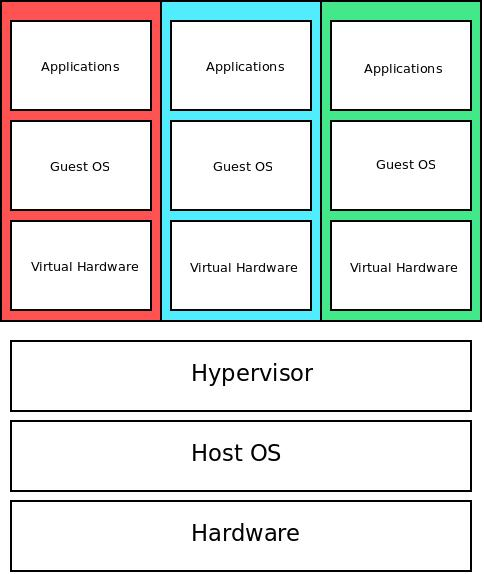
\includegraphics[width=10cm,height=10cm, keepaspectratio]{fullvirt.jpeg}%
  \caption{Full virtualisation architecture}
  \label{fig:full}
\end{figure}

The main advantage of full virtualisation is that it is easy to deploy and should not pose problems to an average user but the virtualisation overhead results in significantly reduced performance when compared to running directly on hardware. Popular examples of full virtualisation applications are Oracle's \textit{VirtualBox}\cite{VirtualBox} and \textit{VMware Workstation}\cite{WorkStation}. 

\subsubsection{Hardware-Layer virtualisation}

Hardware-Layer virtualisation is also a type of full virtualisation, but unlike Type 2 hypervisors, the so called \textit{Type 1 Hypervisors} (also \textit{native} and \textit{bare metal}) run directly on hardware. As seen on figure ~\ref{fig:hardware} there's no Host OS per se. Instead the Guest OSs access to hardware resources is controlled by the hypervisor.

\begin{figure}[ht!]
\centering
  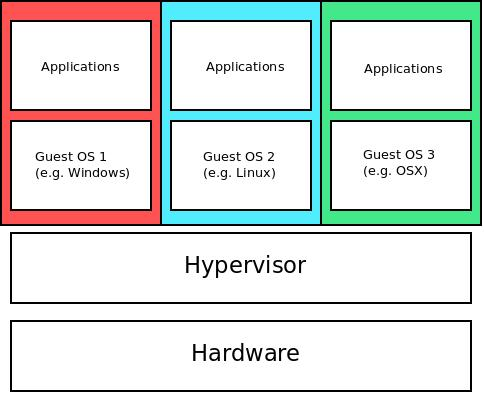
\includegraphics[width=10cm,height=10cm, keepaspectratio]{hwlayer.jpeg}%
  \caption{Hardware-Layer virtualisation architecture}
  \label{fig:hardware}
\end{figure}

Running directly on hardware, Hardware-Layer virtualisation techniques suffer less performance overhead than their OS-layer counterparts. On the other hand, Type 2 hypervisors being essentially applications themselves can be ran in parallel on the host OS whereas Type 1 hypervisors can not. For an average user, setting up a Type 1 hypervisor can be more difficult than Type 2. Commercial examples of Type 1 Hypervisors include Microsoft's \textit{Hyper-V}\cite{hyperv} and VMware's \textit{VSphere} \cite{vsphere}.

\subsubsection{Container-based virtualisation}

Instead of virtualising the underlying hardware, container-based virtualisation also known as OS-Layer virtualisation \cite{taxonomy} focuses on user space and allows running multiple operating systems in parallel as applications using the same kernel as the host operating system. A prime example of a popular container-based virtualisation platform is \textit{Docker} \cite{docker} which leverages on native Linux kernel features to virtualise and isolate OS instances. Figure ~\ref{fig:container} shows a container-based virtualisation architecture in which containerised environments are running operating systems on host OS's kernel. 

\begin{figure}[ht!]
\centering
  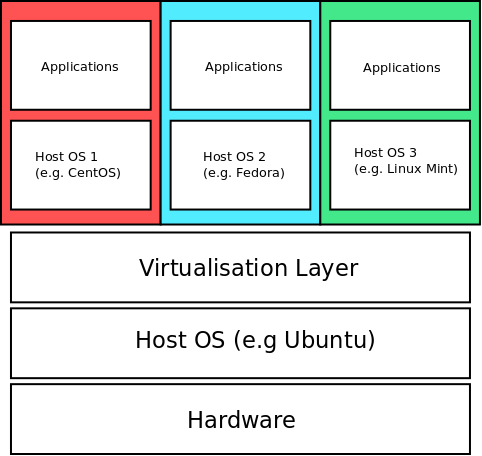
\includegraphics[width=10cm,height=10cm, keepaspectratio]{containers.png}%
  \caption{Container-based architecture}
  \label{fig:container}
\end{figure}

Container-based virtualisation does not need to emulate the hardware as containers communicate directly with the host kernel \cite{eder2016hypervisor} and are thus very fast to start. They also do not require all of the components a fully virtualised environment would need to run and therefore their resource fingerprint is minimal when compared to hypervisor-based virtualisation techniques. \linebreak
The obvious drawback of the technique is that the kernel of the virtualised OS has to be the same as that of Host OS e.g. In a situation depicted in figure ~\ref{fig:container} operating systems based on  Linux kernel could be ran on Ubuntu Host OS but OSs like Windows or OSX could not. On certain virtualisation platforms resource-intensive containers can also affect other containers detrimentally as the shared host OS's kernel is forced to spend its execution time on handling the instructions from the stressed container \cite{Xaviercontainer}.


\subsubsection{Paravirtualisation}

Paravirtualisation differs from full virtualisation by requiring the Guest OS to be modified in order to accomodate the virtual environment in which it is ran. Otherwise the architecture is similar to that of full virtualisation, but with thinner hypervisor allowing performance close to that of a non-virtualised environment. A well-known example of a paravirtualisation hypervisor is \textit{Xen}\cite{xen}.

\subsubsection{Unikernels}

Unikernels are a relatively recent take on virtualising services. Building on the notion that in cloud environments each VM usually specialises to provide only one service even if each VM contains a full-fledged general computer \cite{unikernels}. Unikernels are essentially minimal single-purpose library operating system (\textit{LibOS})\cite{libos} VMs with a single address space. They contain only the minimal set of services, implemented as libraries, built and sealed against modification to run the one application. Unlike the earlier LibOSes unikernels do not require a host OS to run but run directly on a VM hypervisor, such as Xen.

Some benefits of unikernels are obvious. Constructing VMs with minimal set of service libraries results in small images and resource footprints as well as fast boot times. Other benefits include reduced attack surface due to smaller codebase and sealing preventing any code not compiled during the creation of the VM from running. Single-address space improves context switching and eliminates the need for privilege transitions making system calls as efficient as function calls \cite{osv}. Running directly on the hypervisor instead of a host OS eliminates superfluous levels of hardware abstraction.

Optimisation and simplification are not without drawbacks. By definition, unikernels are not intended for general-purpose multi-user computing but for microservice cloud environments. Running multiple applications on a single VM is risky due single-address space does not offer any inherent resource isolation. As unikernels are sealed during compiling, it is not possible to do changes to them afterwards. User is instead required to compile and launch a completely new modified VM.

Popular examples of unikernels are \textit{MirageOS}\cite{mirage} and \textit{OSv}\cite{osv}.

\subsection{Experiment technologies}

This section discusses the technologies used and studied in the experiment in more detail. Virtualisation technologies are Docker, Xen, KVM and OSv and they are run on an OpenStack testbed.

\subsubsection{Openstack}

Openstack \cite{openstackproject} is an open-source software platform for cloud computing. A project originally founded by NASA and Rackspace Inc. now has a large base of supporting companies  \cite{openstackpartners} and a thriving community.
	Openstack allows its users to deploy a full-fledged cloud computing infrastructure. User can control pools of both physical and virtual computing, storage and networking resources. It can be run on commodity hardware and supports a plethora of enterprise- and open source technologies making it possible to use heterogeneous physical and software environments.
	Openstack consists of different projects that provide services for the system. A user can freely choose which services to deploy. Project range from essential \textit{Core Services} like computing, block storage, identity service and networking to more specific and specialised such as MapReduce and Bare-metal provisioning\cite{openstackproject}. Openstack boasts many features: It is massively scalable supporting up to million physical and 80 million virtual machines \cite{openstack}. It also supports a wide array of market-leading virtualisation technologies such as QEMU, KVM and Xen and it is fully open-source with thriving community and industry backing \cite{openstackpartners}. Other features include fine-grained access control and multi-tenancy, fault-tolerance and self-healing \cite{openstackfeatures}.


\subsubsection{Cloudify}

Cloudify \cite{cloudify} is an open-source orchestration software aiming to provide a unified control and modelling layer for common cloud computing platforms. Cloudify can be used to uniformly orchestrate heterogeneous sets of both virtual and physical cloud resources such as networking, computing and storage resources. They can also be provided from different environments such as OpenStack, AWS, Google Cloud Platform (GCP), Kubernetes and even bare-metal clouds. Orchestrating different versions of the same underlying cloud environment is also possible. The applications, workflows and the cloud infrastructure itself is described with OASIS TOSCA \cite{Tosca} based Domain Specific Language (DSL) in configuration files called \textit{blueprints} in Cloudify jargon. Configuration files are vendor-agnostic, meaning the same configuration can be reused with different underlying infrastructure. Cloudify \textit{plugins} act as an abstraction layer between the generic blueprints and cloud environments' more speclialised APIs. The generalising approach makes cloudify suitable for hybrid clouds and allows seamless migration of resources between different environments.

\subsubsection{Comparison of Openstack and Cloudify}

Both Openstack and Cloudify are used to operate a large number of computing, networking and storage resources. However, they are not directly comparable. While Cloudify can be used to orchestrate resources and applications on a cloud platform, OpenStack is a cloud platform. Similar orchestration project within OpenStack is Heat \cite{heat}, which can be used similarly to Cloudify's DSL to write human-readable templates (\textit{HOTs -- Heat Orchestration Templates} as they are called in the Heat project) to automate deployments of applications and cloud resources. Heat orchestration is of course limited to OpenStack itself. Even though there are drivers which allow OpenStack to manage resources from major public clouds such as AWS and GCP (and thus allowing a public/private hybrdi cloud), the resources are abstracted to those common to OpenStack: Heat cannot orchestrate them independently of an OpenStack deployment. Cloudify however is cloud-platform agnostic and it can manage multiple different cloud environments simultaneously, including OpenStack. On the subject of hybrid clouds, Cloudify supports bare-metal deployments by default and OpenStack's project \textit{Ironic} for provisioning bare-metal instances has  been integrated to OpenStack since 'Kilo' development cycle. 



\subsubsection{Docker}
\subsubsection{Xen}
\subsubsection{KVM}
\subsubsection{OSv}

